\chapter{Screenshots der implementierten Benutzerschnittstelle}\label{ah:abbildungen}

\begin{figure}[H]
	\centering 
	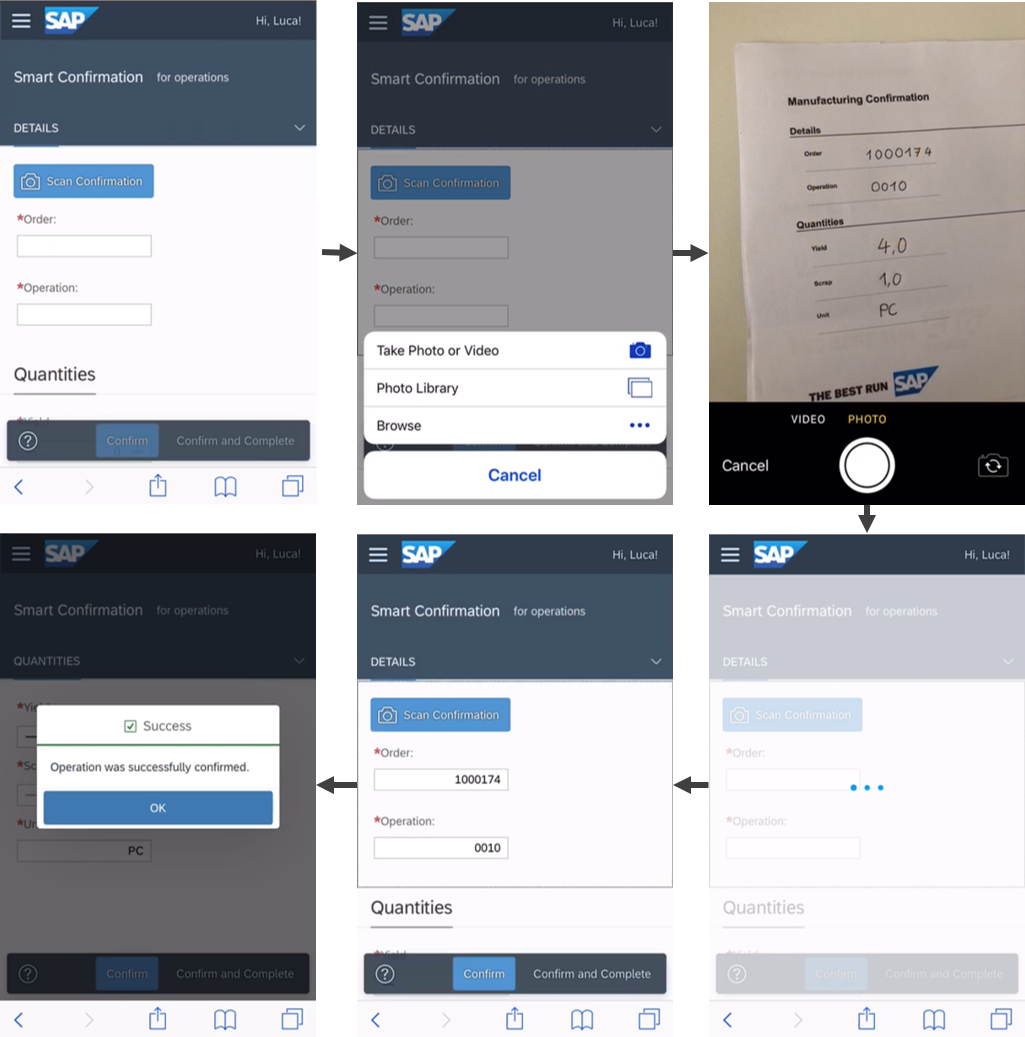
\includegraphics[width=\textwidth]{img/ablauf_ocr.png}	
	\caption[Eingabemaske zur Rückmeldung via Texterkennung]{\label{fig:Eingabemaske zur Rückmeldung via Texterkennung}Ablauf der Rückmeldung durch Texterkennung
	}
\end{figure}

\begin{figure}[H]
	\centering 
	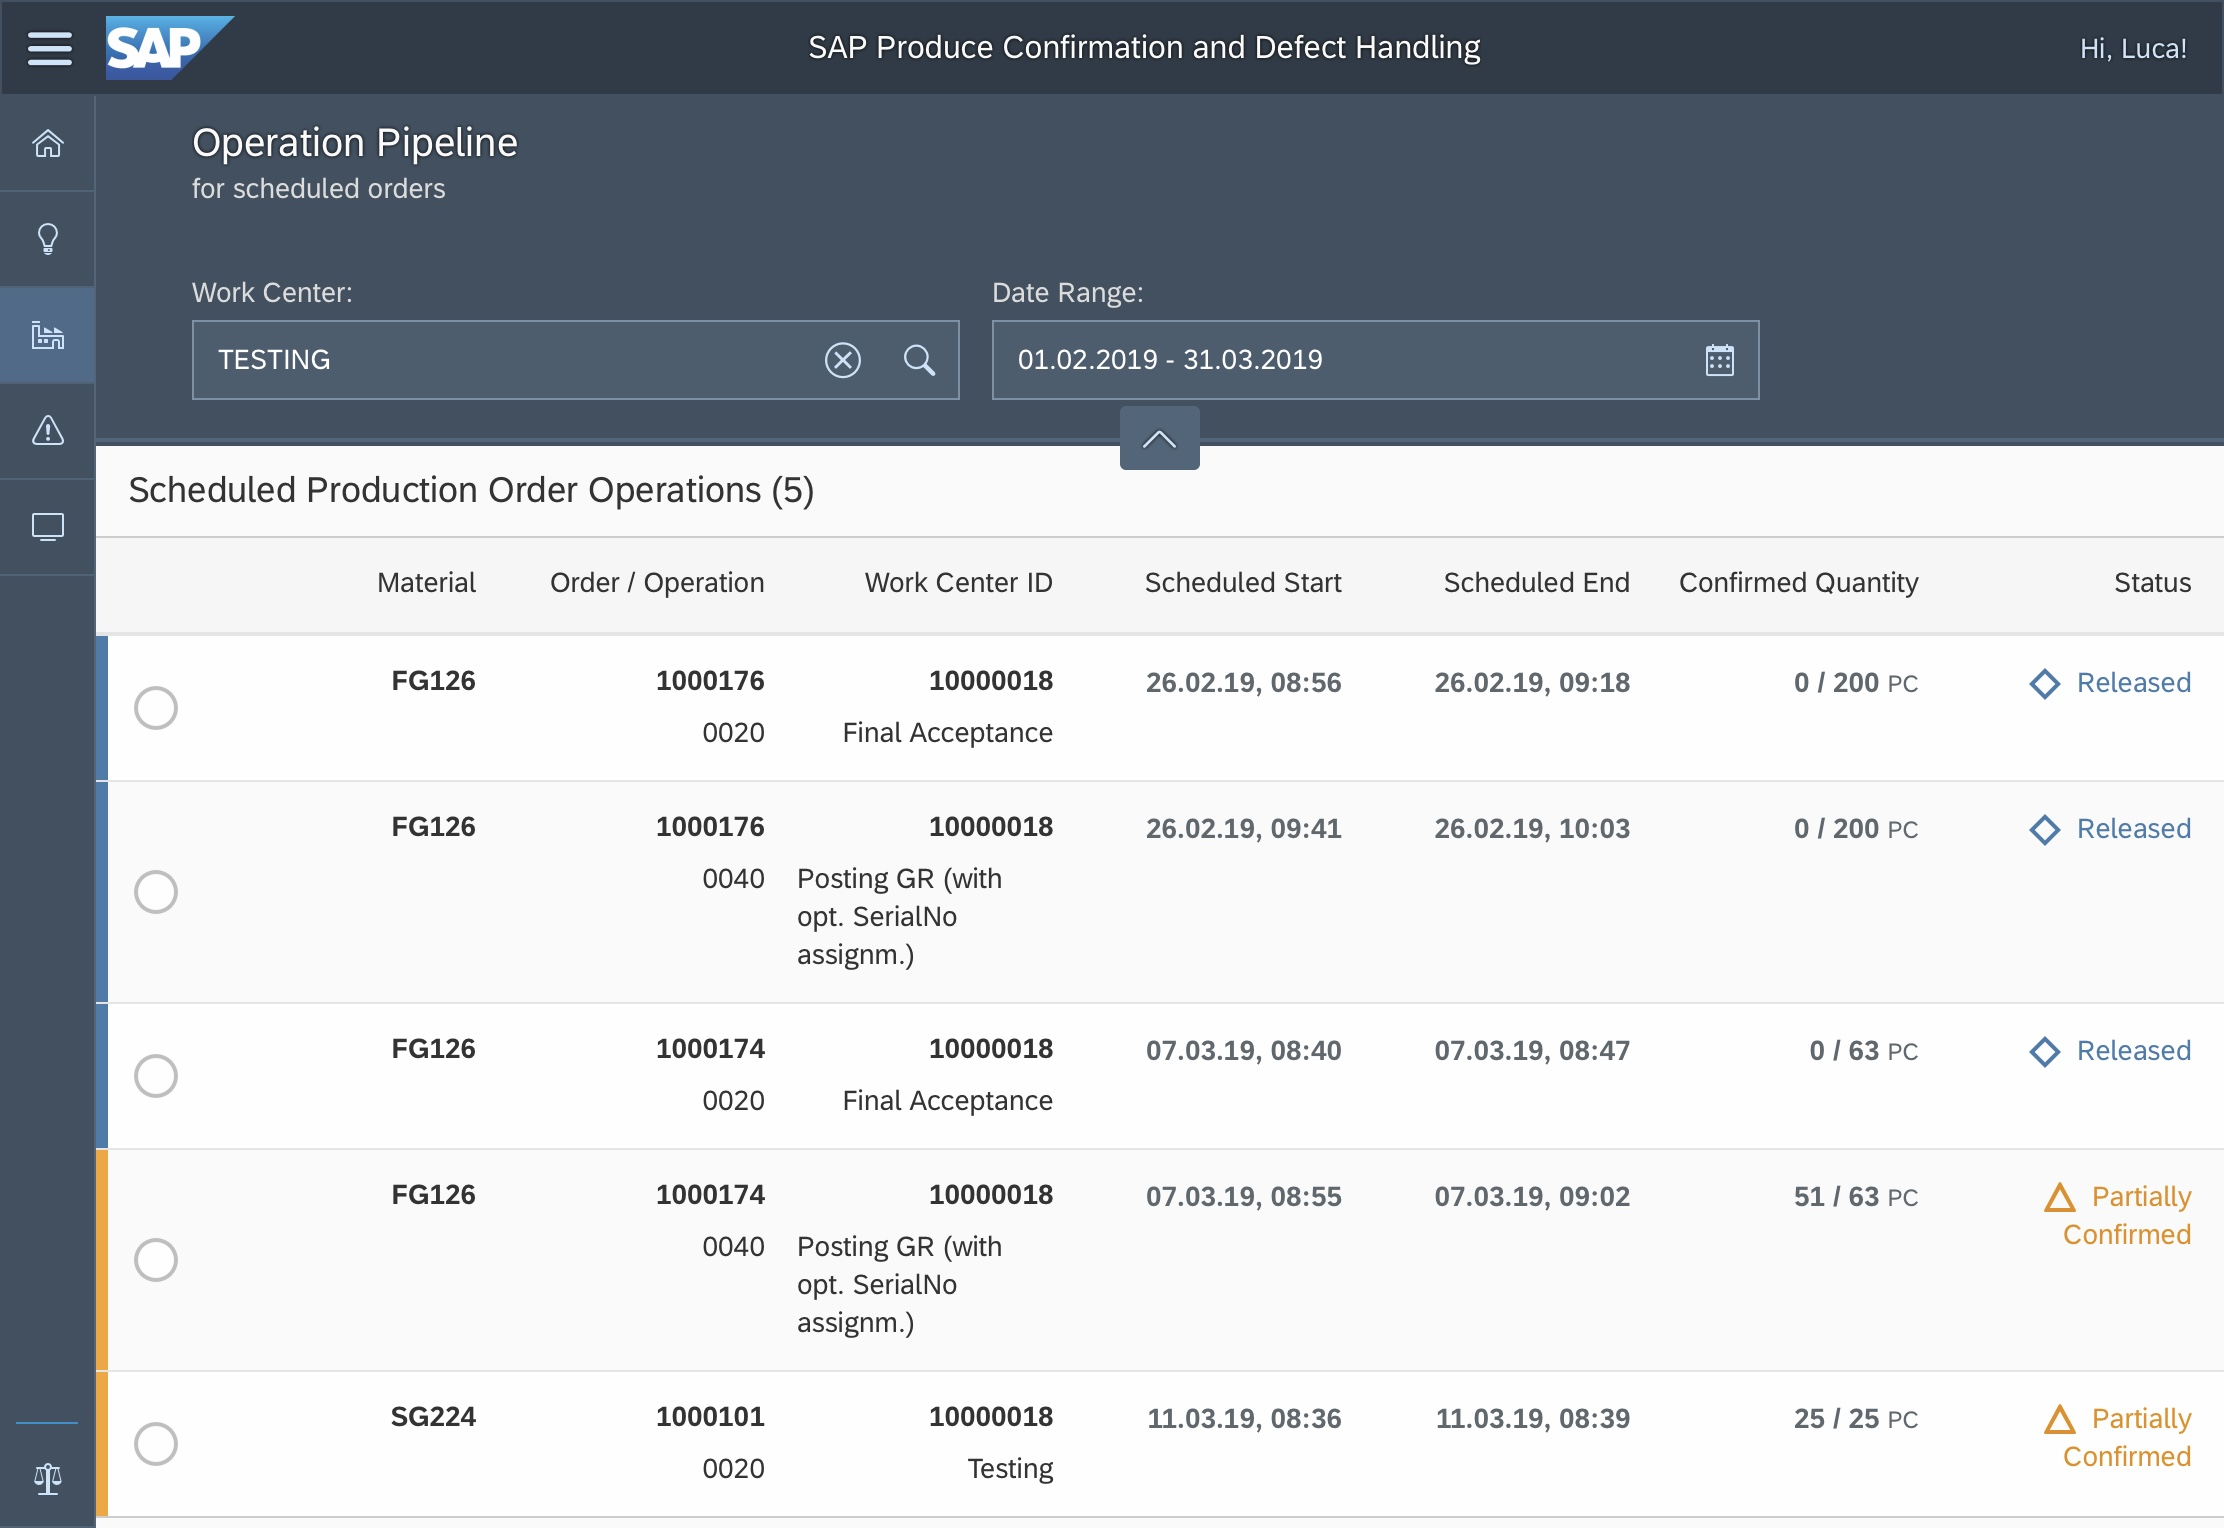
\includegraphics[width=1.2\textwidth, angle =90 ]{img/Arbeitsvorrat.jpg}	
	\caption[Übersicht des Arbeitsvorrats (ohne Buttons)]{\label{fig:arbeitsvorrat}Übersicht des Arbeitsvorrats 
	}
\end{figure}
\begin{figure}[H]
	\centering 
	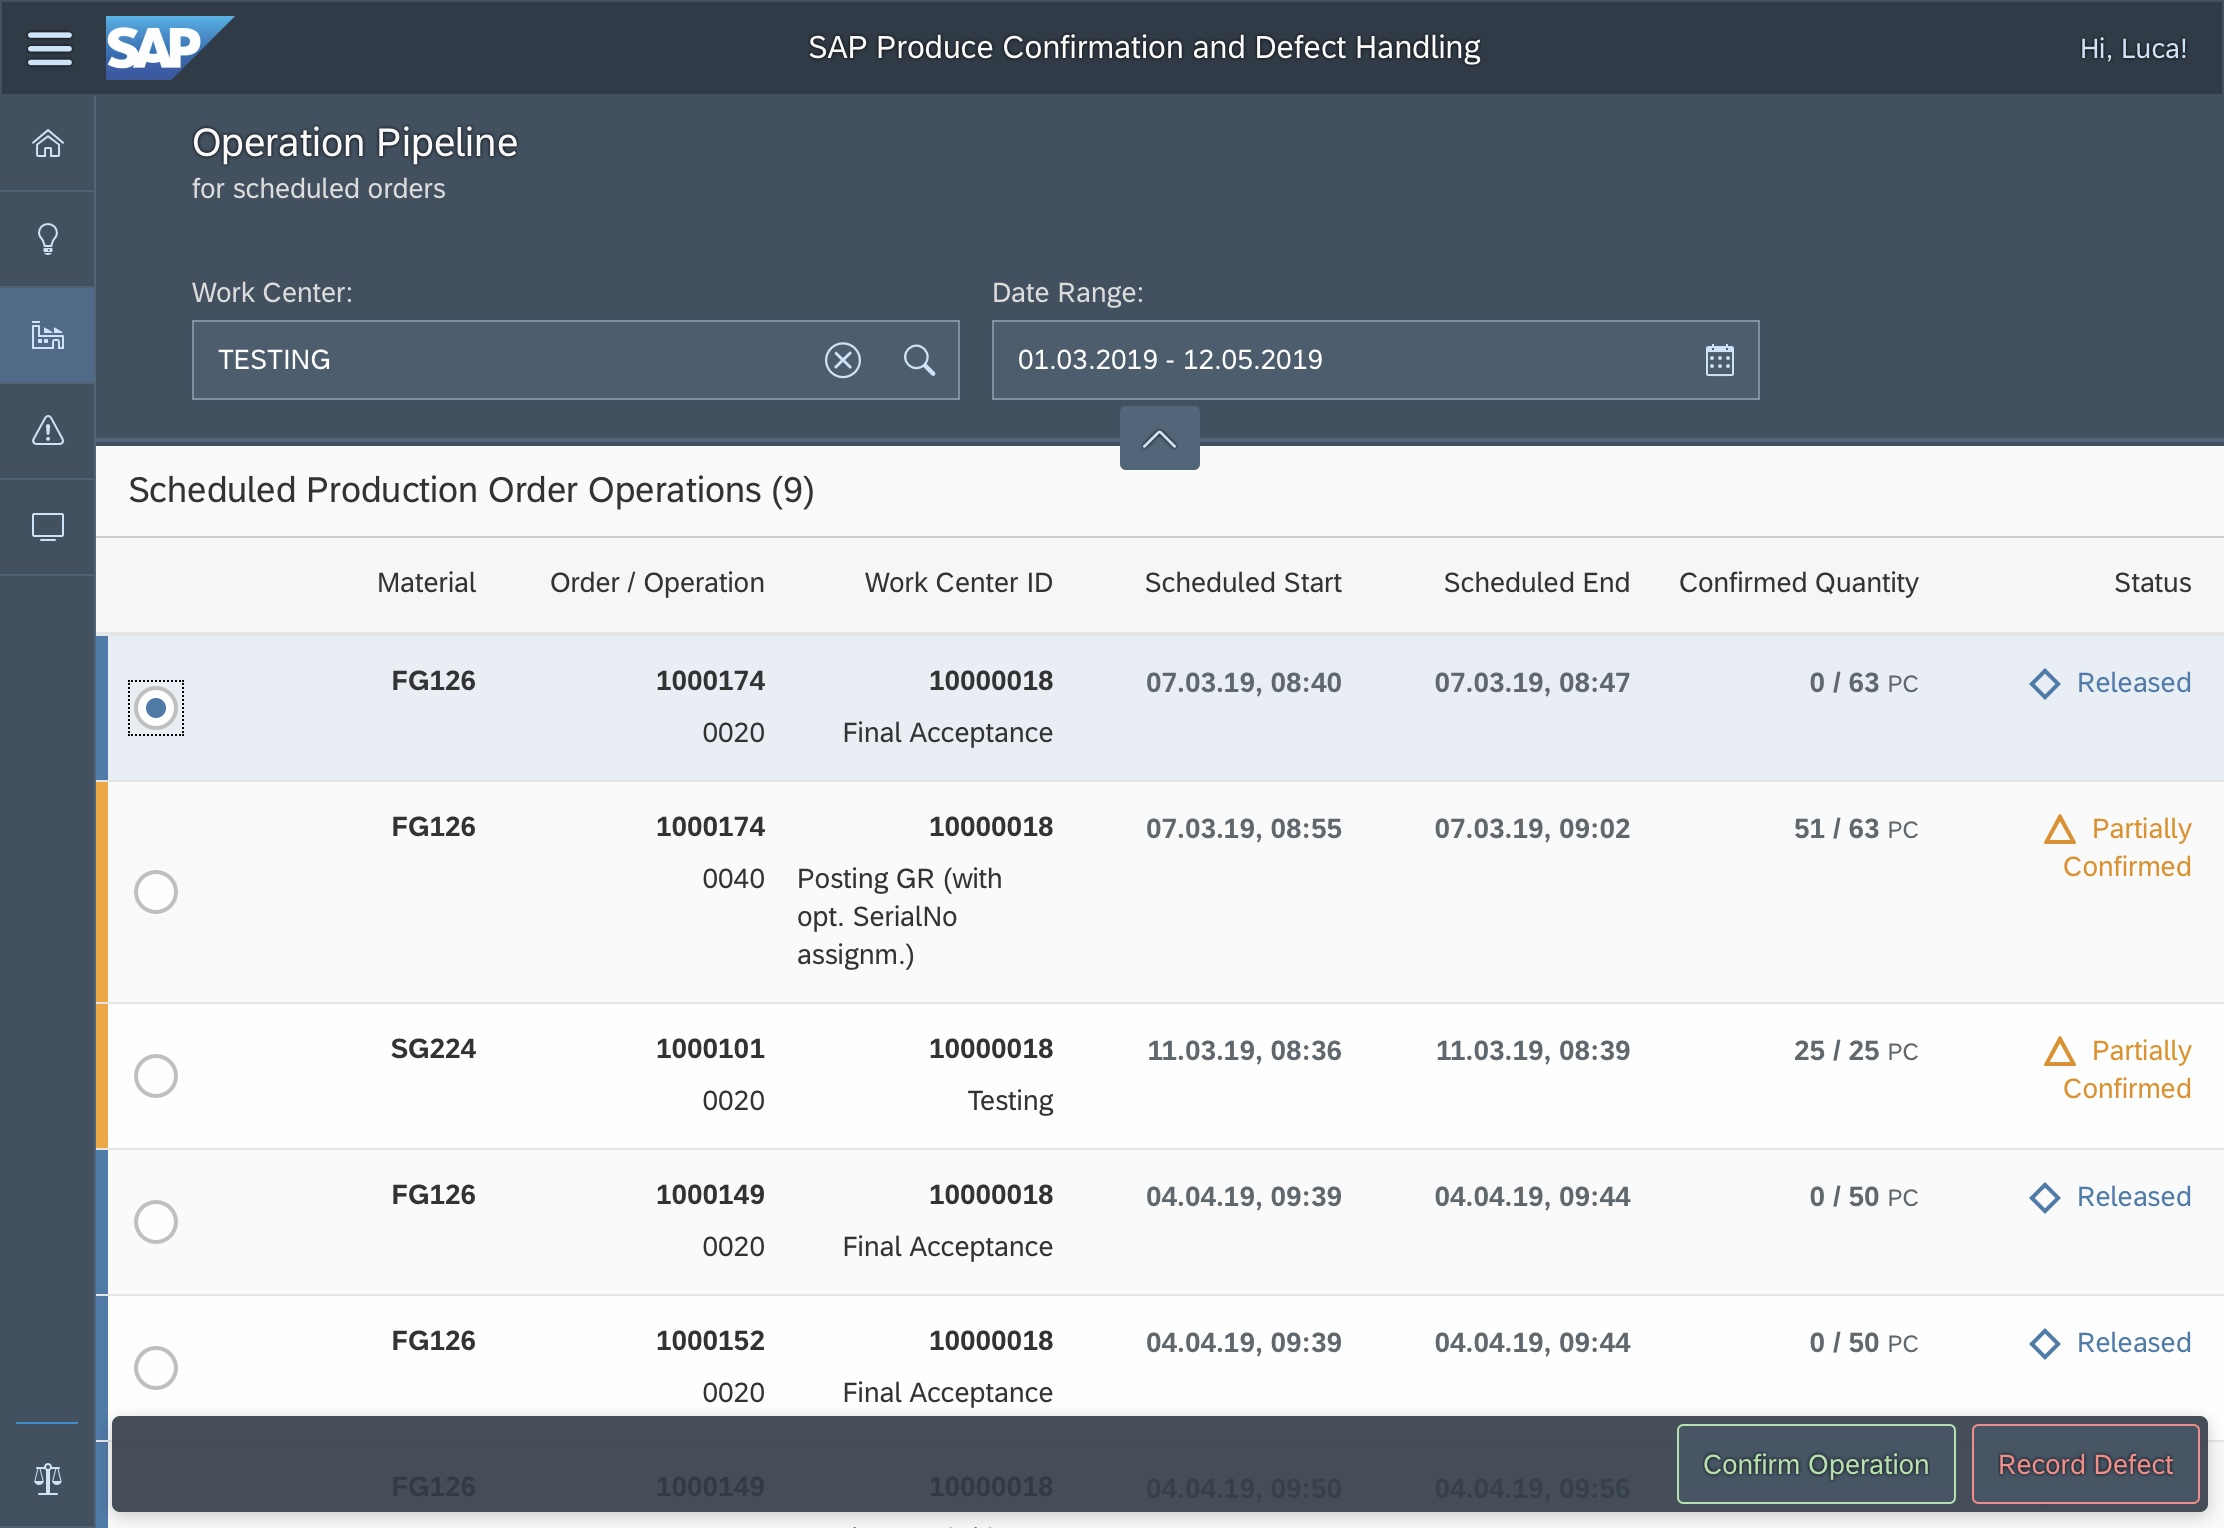
\includegraphics[width=1.2\textwidth, angle =90 ]{img/Arbeitsvorrat mit buttons.jpg}	
	\caption[Übersicht des Arbeitsvorrats (mit Buttons)]{\label{fig:arbeitsvorrat2}Übersicht des Arbeitsvorrats (mit Rückmelde- und Defekterfassungsoptionen)
	}
\end{figure}


\begin{figure}[H]
	\centering 
	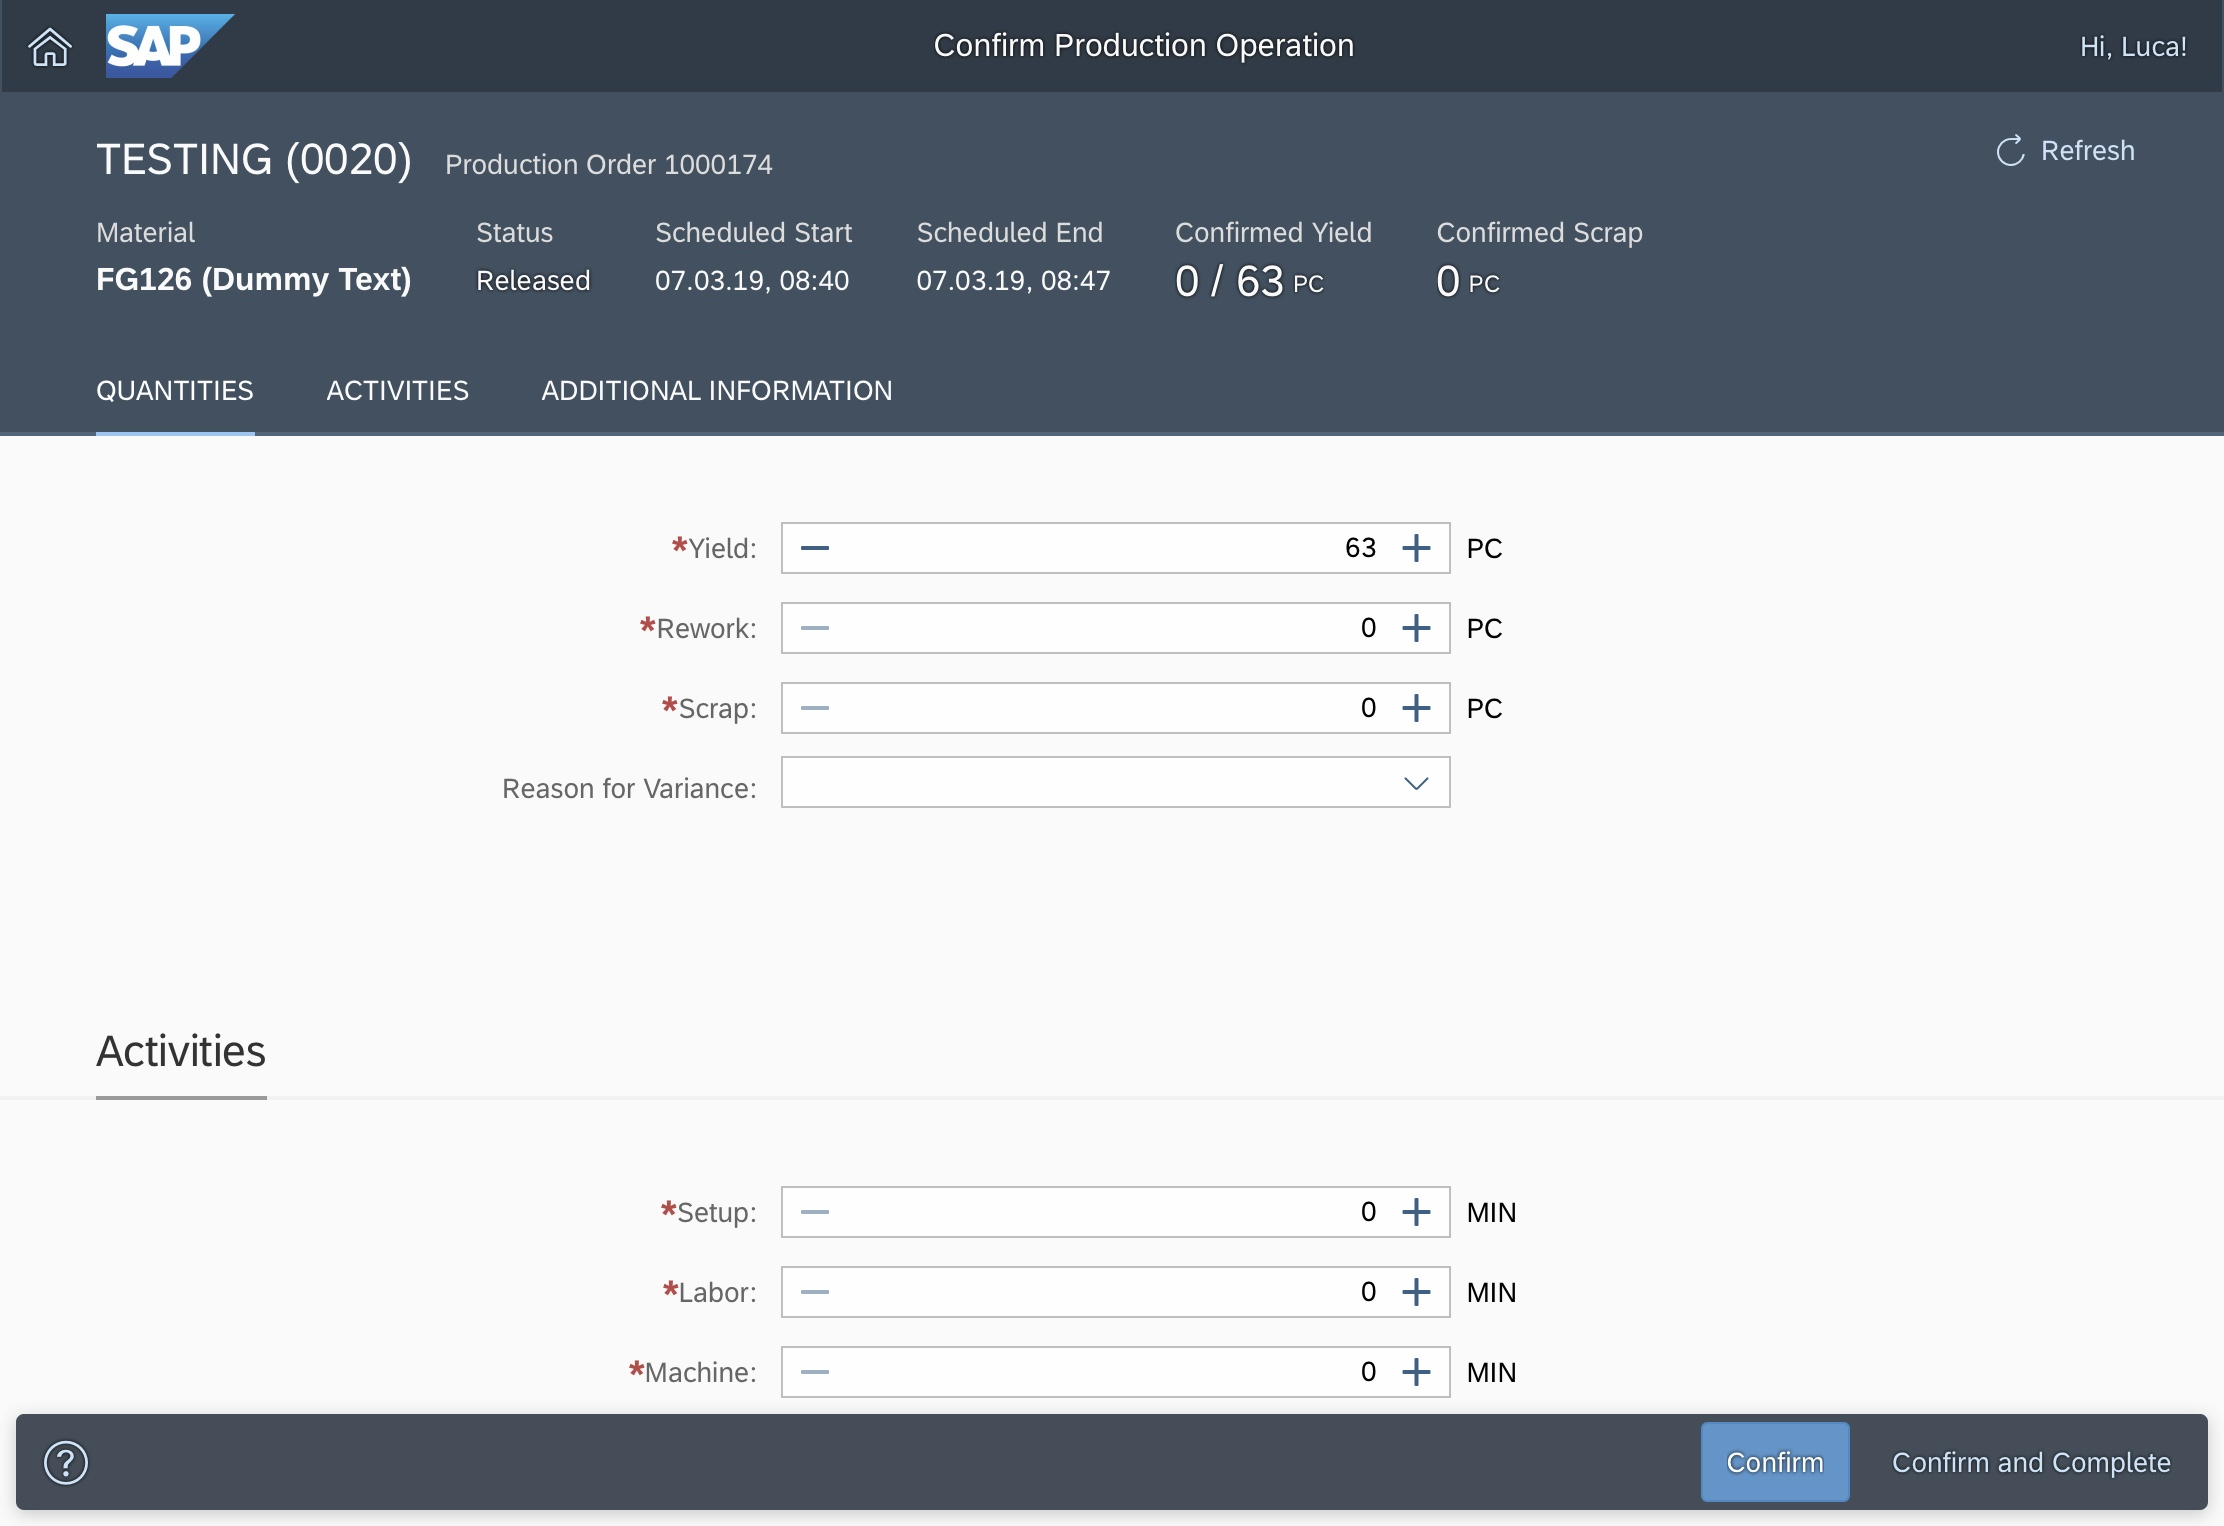
\includegraphics[width=1.2\textwidth, angle =90 ]{img/confirm.jpg}	
	\caption[Eingabemaske zur Erfassung von Rückmeldungen]{\label{fig:Eingabemaske zur Erfassung von Rückmeldungen}Eingabemaske zur Erfassung von Rückmeldungen
	}
\end{figure}
\begin{figure}[H]
	\centering 
	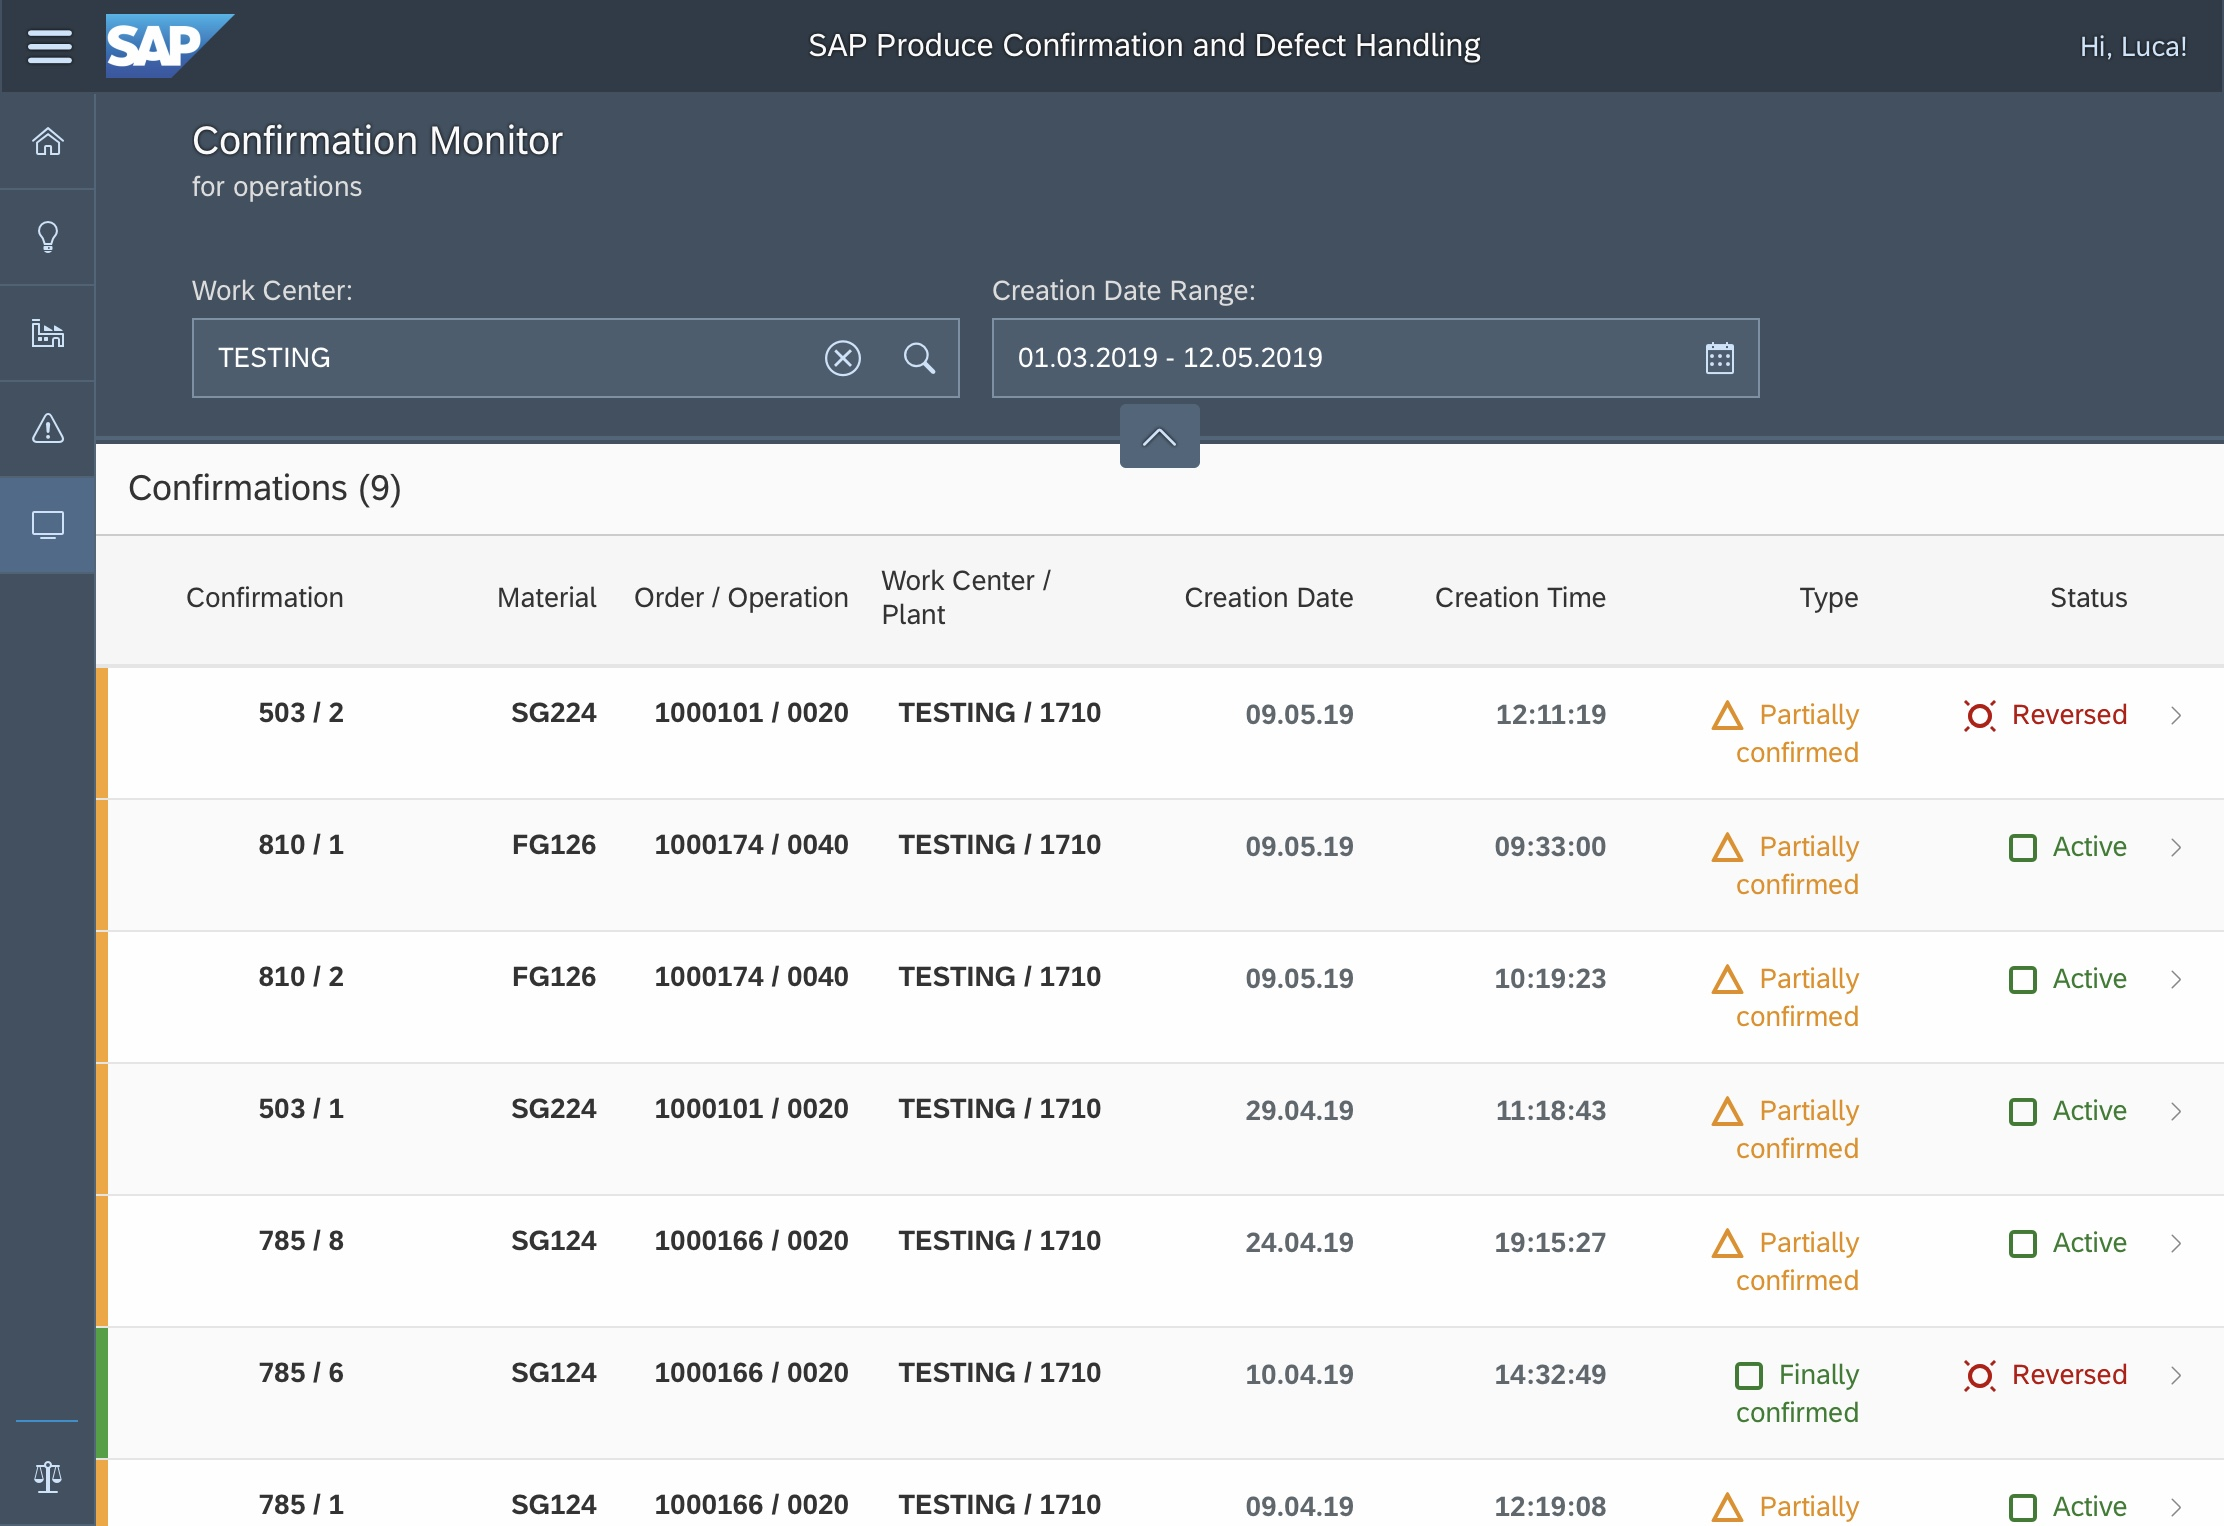
\includegraphics[width=1.2\textwidth, angle =90 ]{img/confmonitor.jpg}	
	\caption[Übersicht der Rückmeldungen]{\label{fig:Überischt der Rückmeldungen}Übersicht der Rückmeldungen
	}
\end{figure}
\begin{figure}[H]
	\centering 
	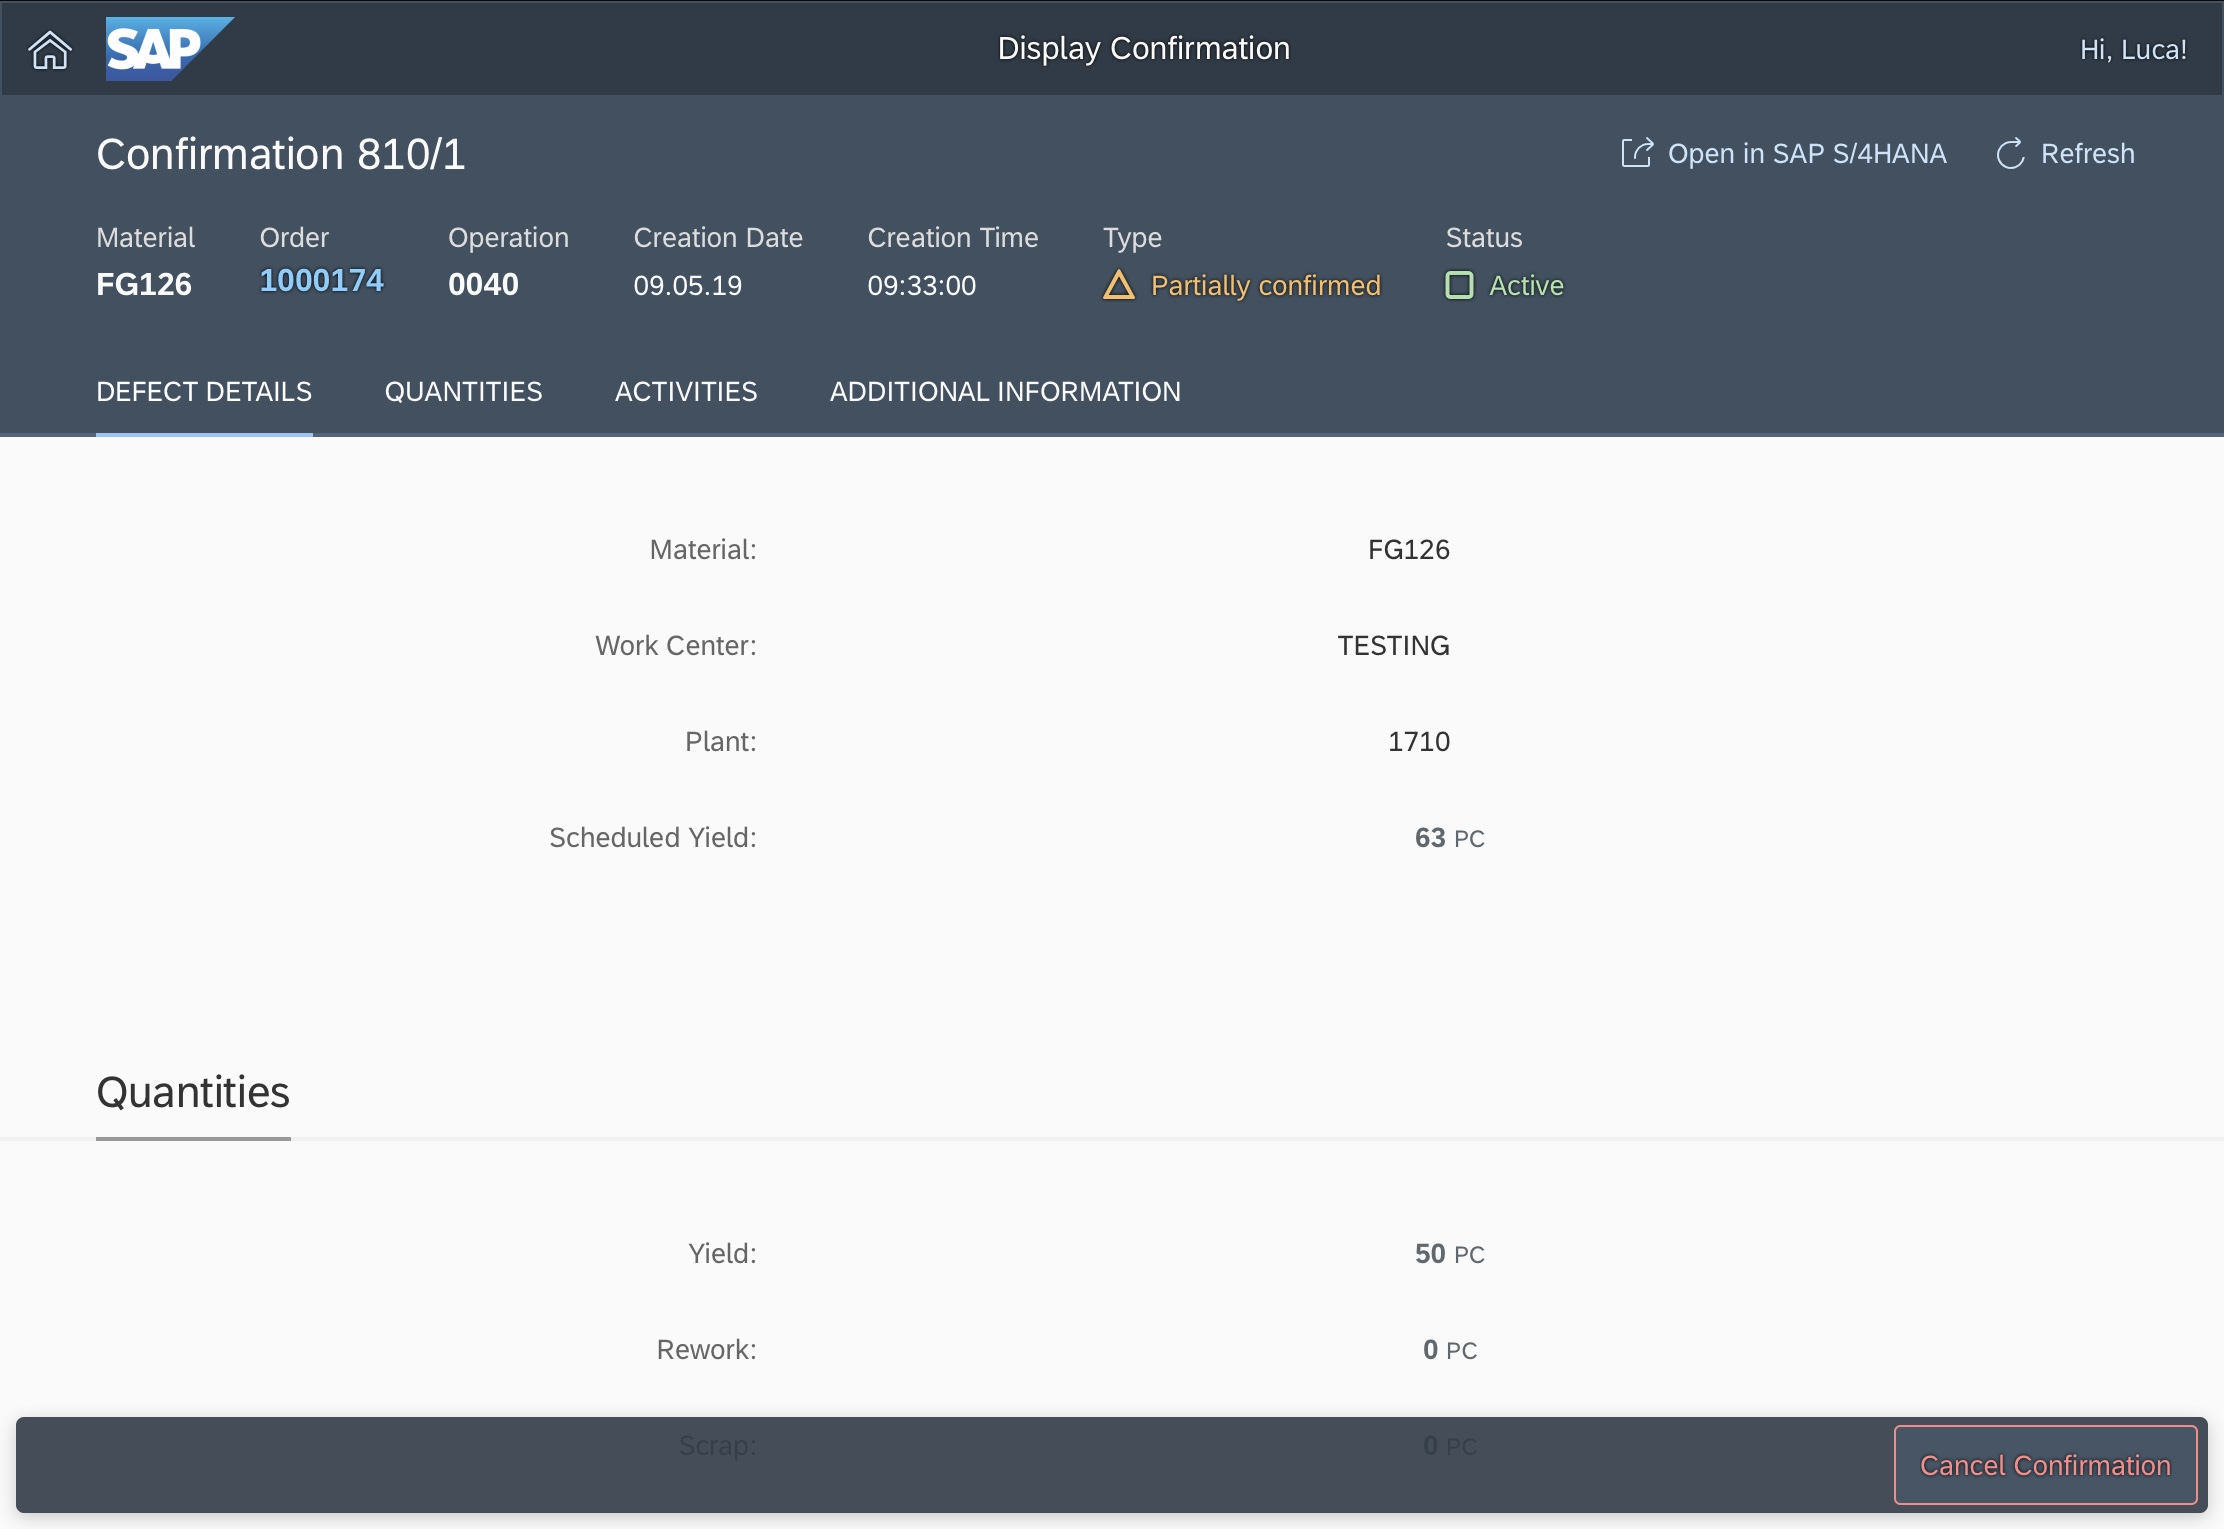
\includegraphics[width=1.2\textwidth, angle =90 ]{img/stornieren.jpg}	
	\caption[Detailansicht einer Rückmeldung]{\label{fig:Detailansicht einer Rückmeldung}Detailansicht einer Rückmeldung
	}
\end{figure}
\begin{figure}[H]
	\centering 
	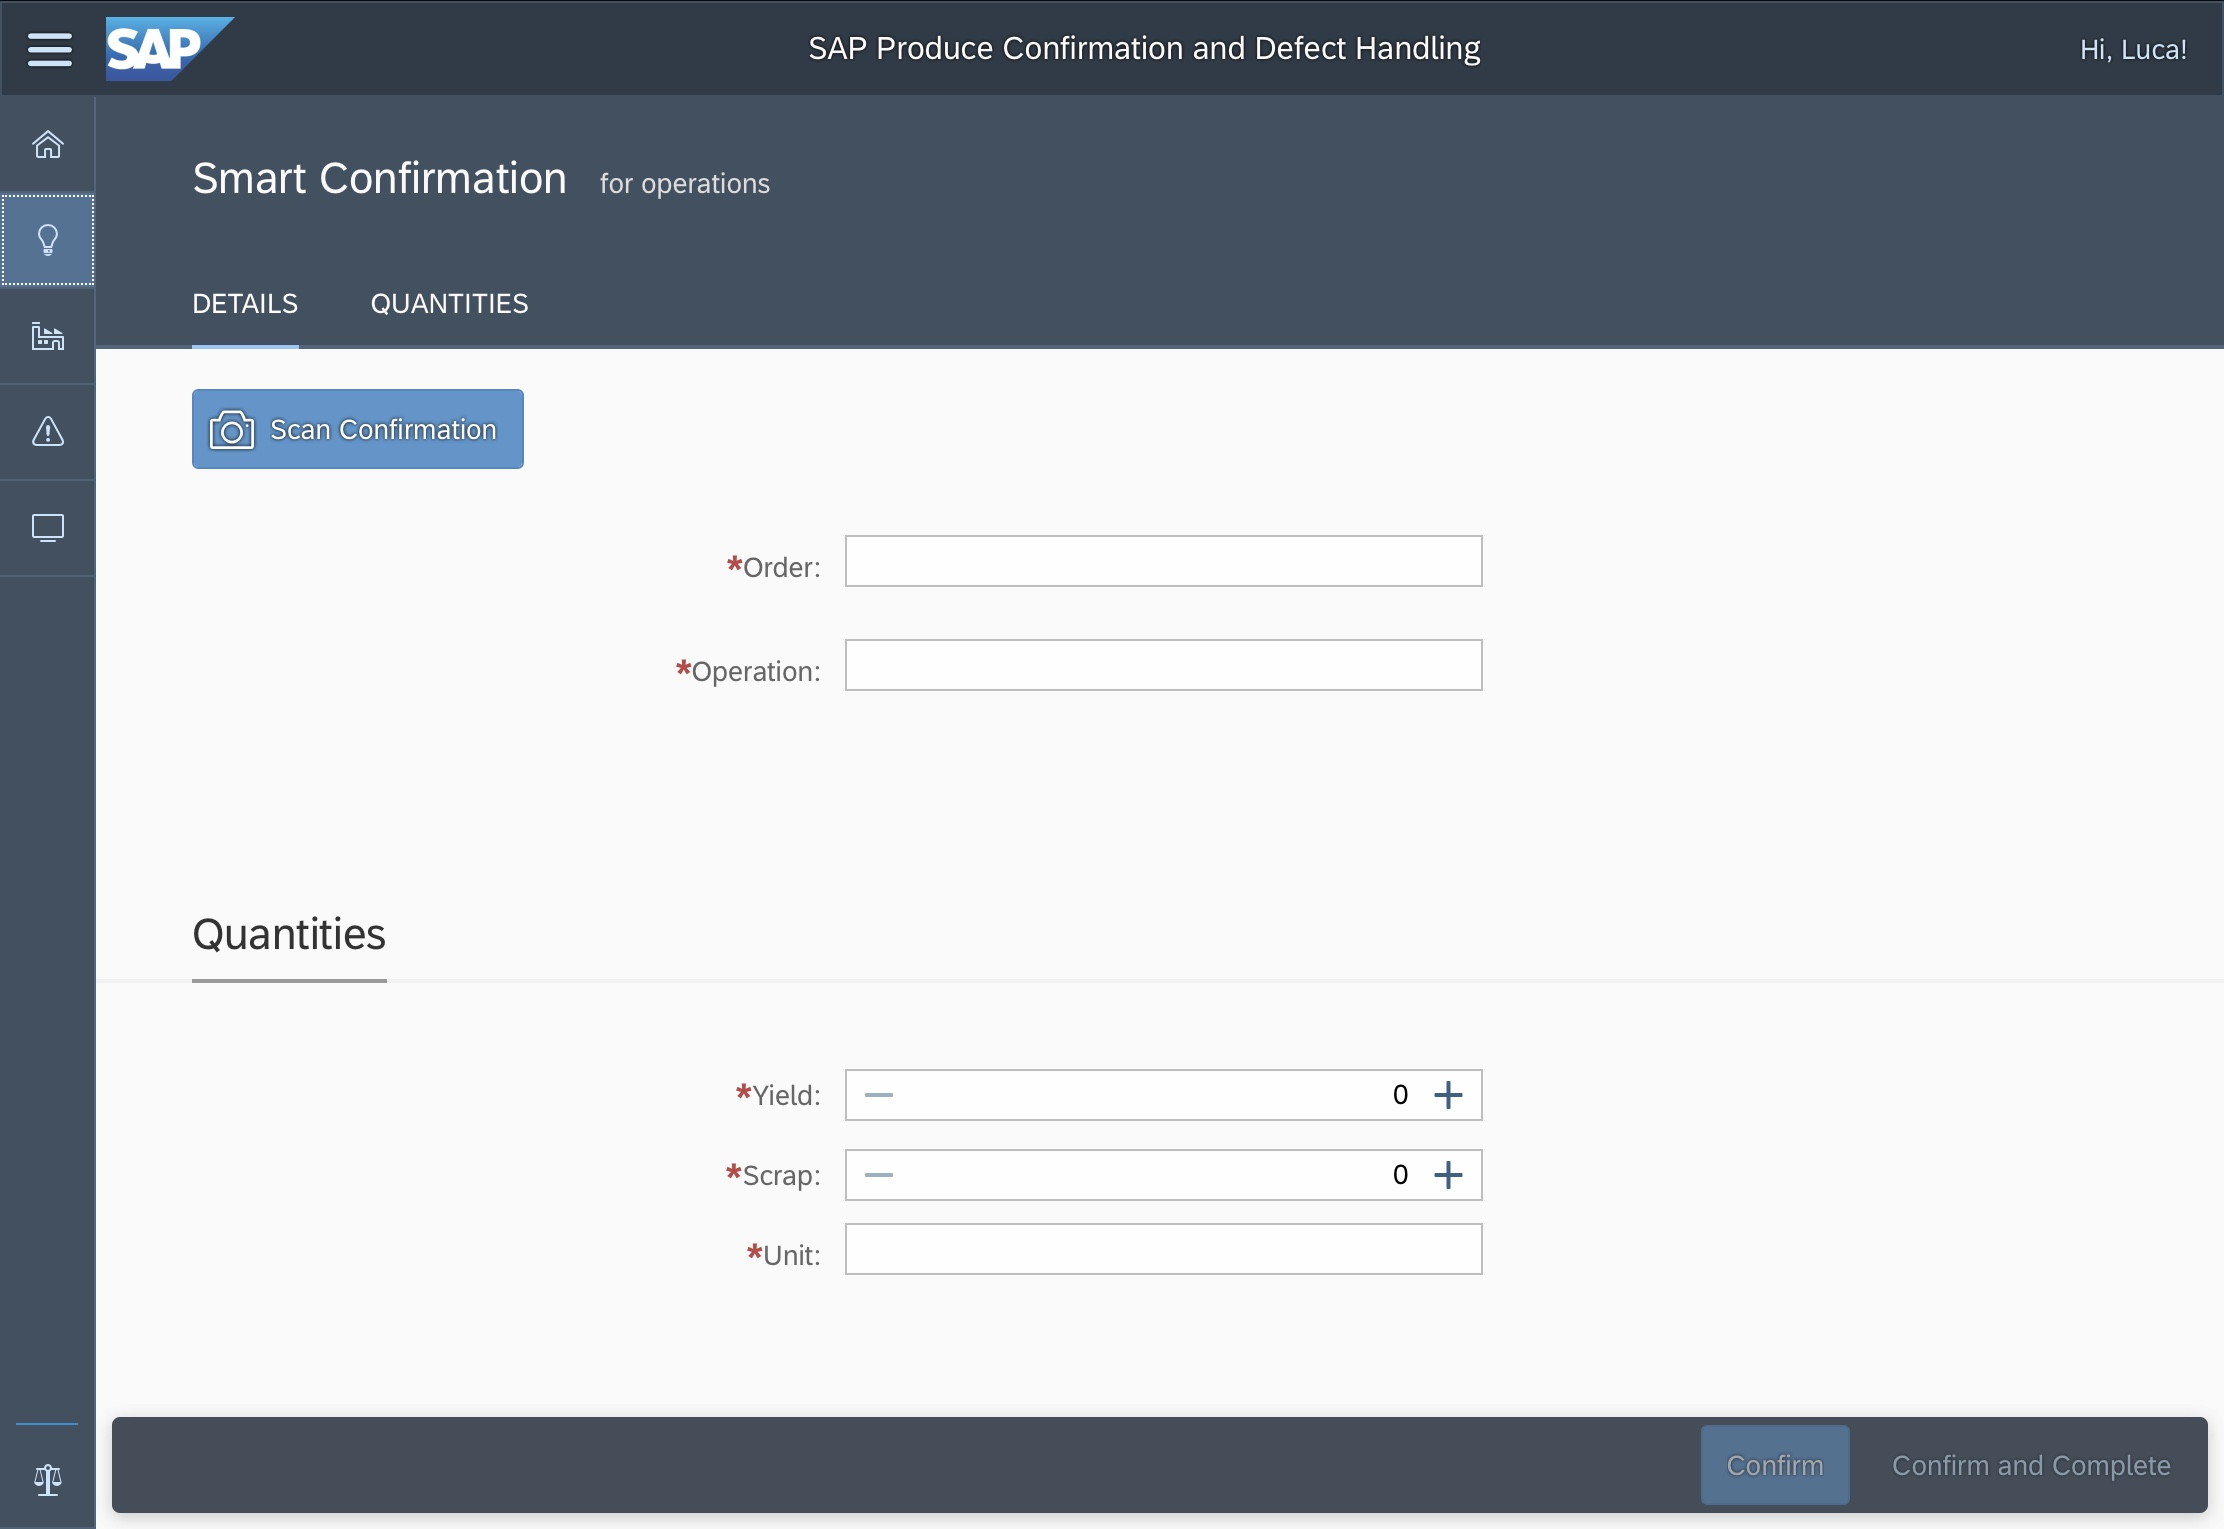
\includegraphics[width=1.2\textwidth, angle =90 ]{img/scanner.jpg}	
	\caption[Eingabemaske zur Rückmeldung via Texterkennung]{\label{fig:Eingabemaske zur Rückmeldung via Texterkennung}Eingabemaske zur Rückmeldung via Texterkennung
	}
\end{figure}


\begin{figure}[H]
	\centering 
	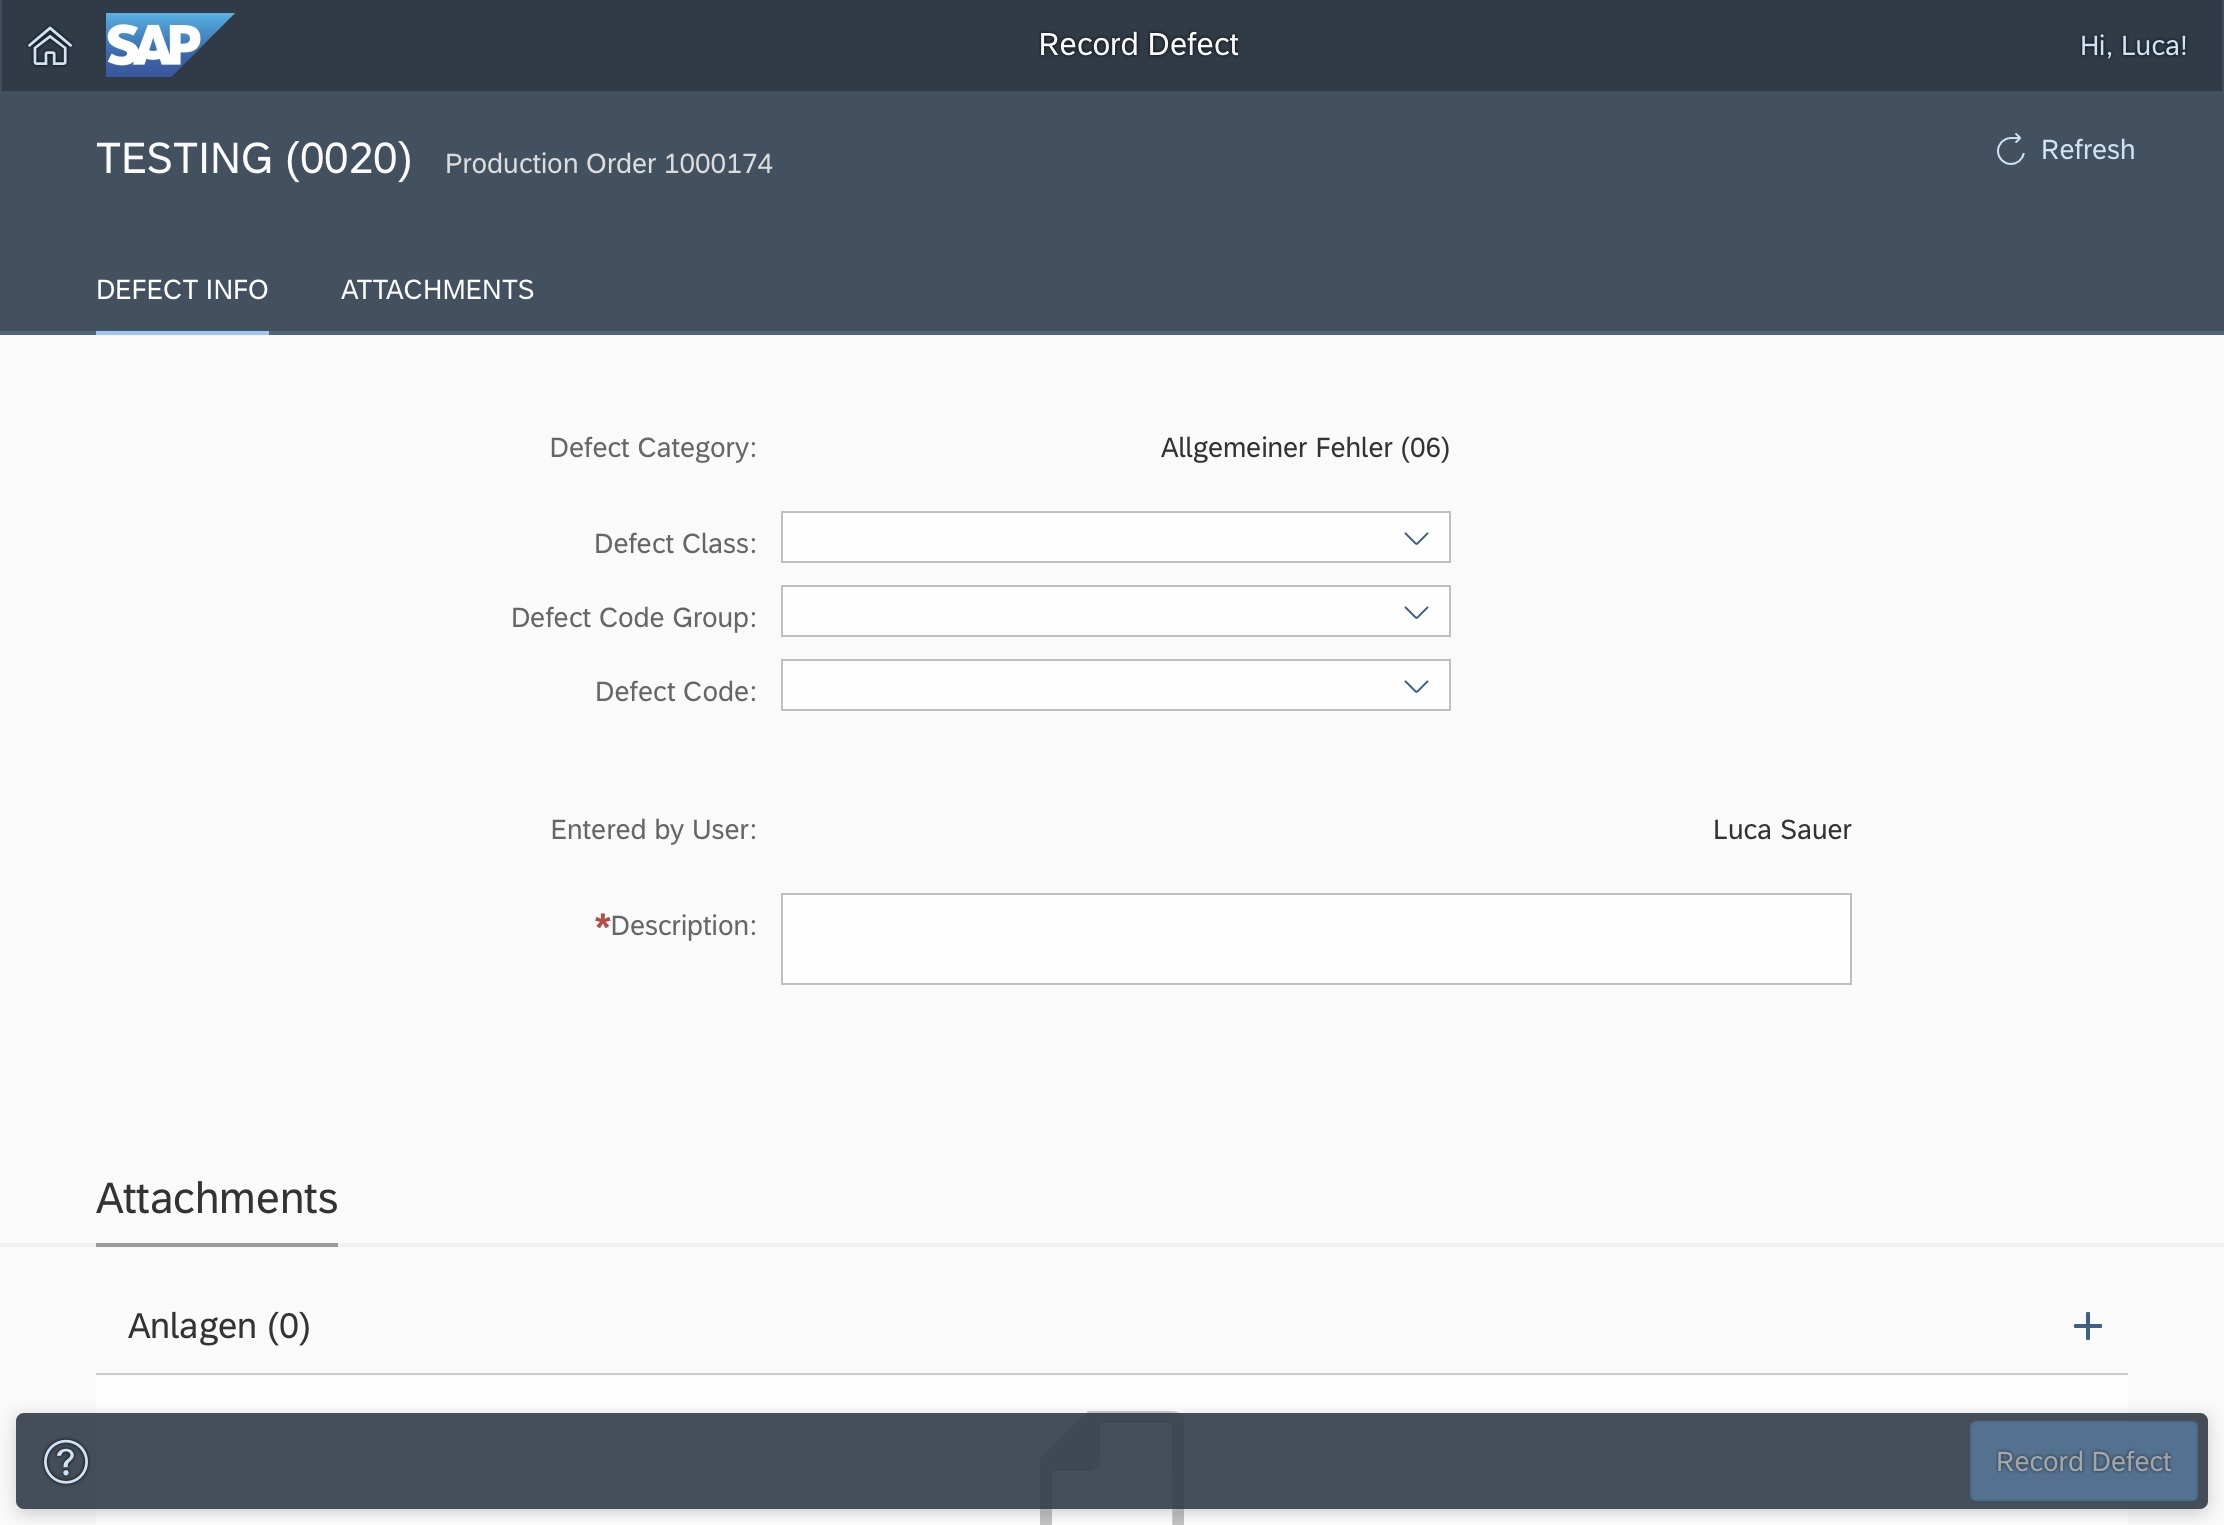
\includegraphics[width=1.2\textwidth, angle =90 ]{img/defectrecord.jpg}	
	\caption[Eingabemaske zur Erfassung von Defekten]{\label{fig:Eingabemaske zur Erfassung von Defekten}Eingabemaske zur Erfassung von Defekten
	}
\end{figure}

\begin{figure}[H]
	\centering 
	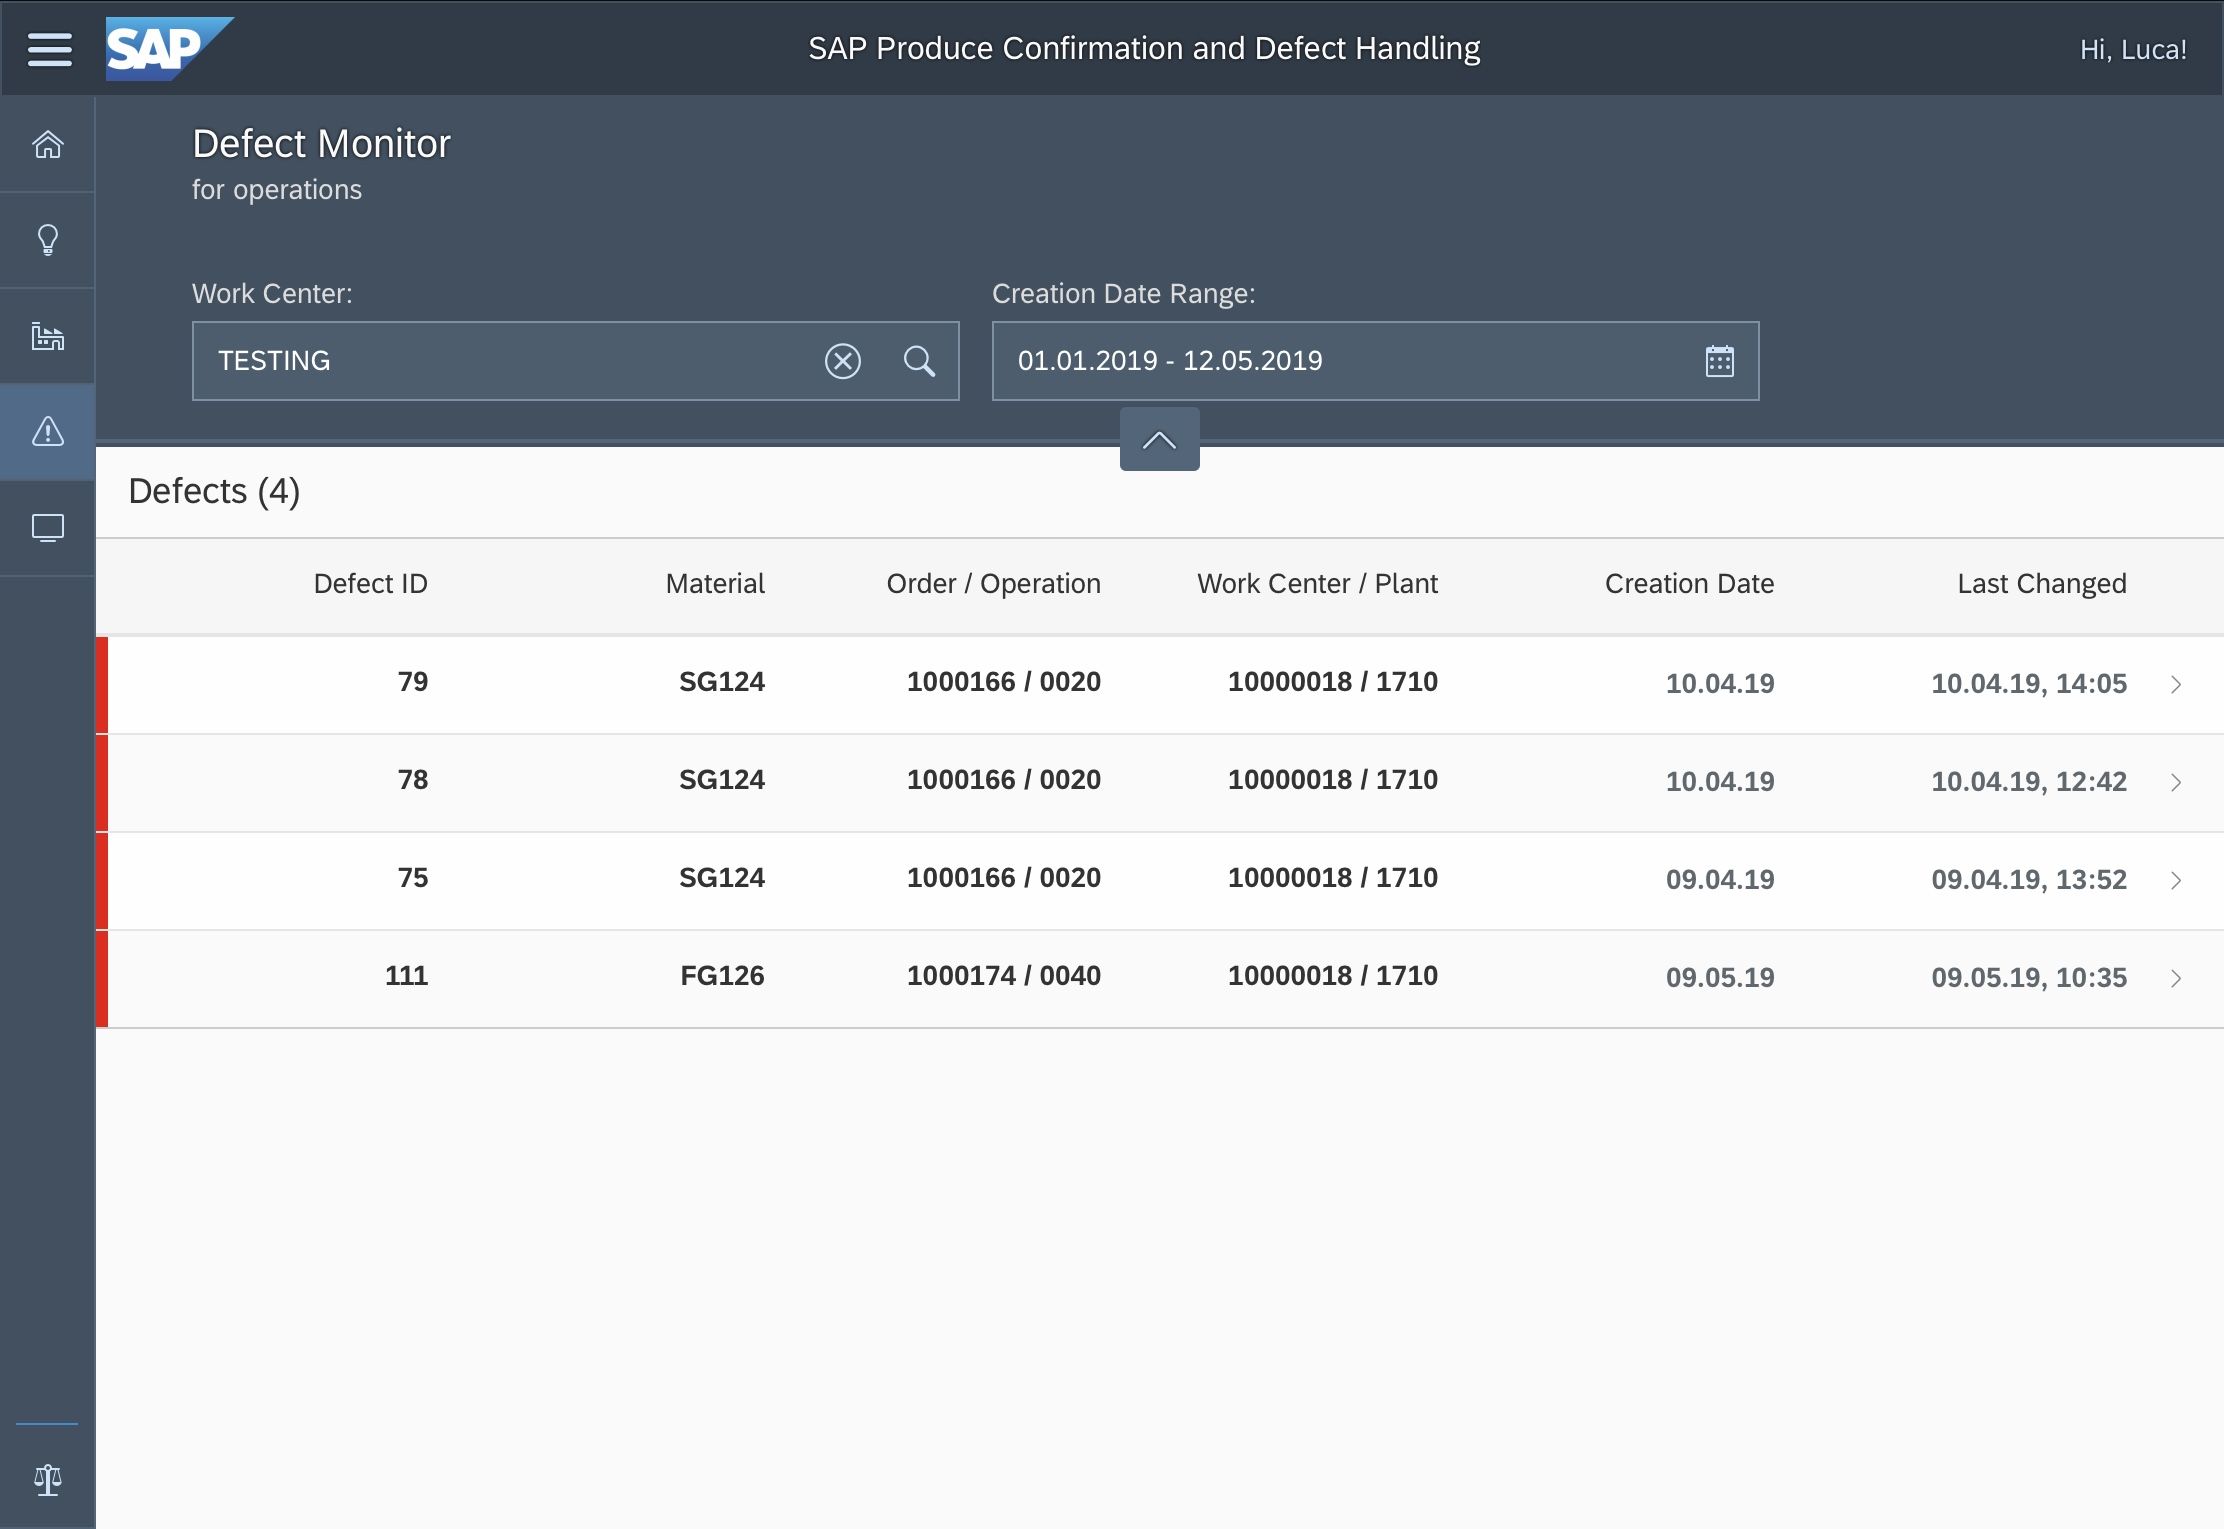
\includegraphics[width=1.3\textwidth, angle =90 ]{img/defectmonit.jpg}	
	\caption[Übersicht der Defekte]{\label{fig:Übersicht der Defekte}Übersicht der Defekte
	}
\end{figure}
